\documentclass[a4paper,article,14pt]{extarticle}

\usepackage{audiploma}
\usepackage{euscript}
\usepackage{longtable}
\usepackage{makecell}
\usepackage[pdftex]{graphicx}
\usepackage{amsthm,amssymb, amsmath}
\usepackage{textcomp}
\usepackage[style=numeric-comp, sorting = none]{biblatex}
\usepackage{csquotes}
\addbibresource{references.bib}

\begin{document}

% --------------------- Стандарт СПб АУ РАН --------------------------%

\begin{titlepage}

\newgeometry{left=30mm, top=30mm, right=15mm, bottom=30mm, nohead, nofoot}

\vspace{15mm}
\begin{center}
    
\includegraphics[width = \textwidth]{images/autitle.png}
\end{center}

\vspace{0.1mm}

\begin{flushright}
    «\rule{1cm}{0.15mm}» \rule{2cm}{0.15mm} 2021г. \\
    Зав. каф. \\
    Теоретической физики \\
    \rule{25mm}{0.20mm} д.ф.-м.н. С. А. Тарасенко \\
\end{flushright}


\begin{center}

\vspace{9mm}
\textbf{\large ИСПОЛЬЗОВАНИЕ ТУЛИЕВЫХ БОЛОМЕТРОВ В КАЧЕСТВЕ ПЕРЕСПЕКТИВНЫХ ДЕТЕКТОРОВ СОЛНЕЧНЫХ АКСИОНОВ}
\vspace{9mm}

выпускная квалификационная работа бакалавра \\
\vspace{10mm}
Направление 03.03.01 Прикладные математика и физика \\
\vspace{14mm}
\textbf{\large Кузьмичев Артем Михайлович}


\vspace{16mm}

% Научный руководитель
\textbf{Научный руководитель} \hfill \rule{6.5cm}{0.15mm} Е.В. Унжаков \\
\vspace{5mm}
\textbf{Студент} \hfill  \rule{6cm}{0.15mm} А.М. Кузьмичев

\vfill 

{Санкт-Петербург, 2021}
\end{center}
\end{titlepage}
% Возвращаем настройки geometry обратно (то, что объявлено в преамбуле)
\restoregeometry
% Добавляем 1 к счетчику страниц ПОСЛЕ titlepage, чтобы исключить
% влияние titlepage environment
\addtocounter{page}{1}
\tableofcontents
\pagebreak


\specialsection{Введение}

В настоящее время Стандартная модель является наиболее успешной физической теорией, описывающей элементарные частицы и их взаимодействия. Тем не менее, существует целый ряд наблюдений и экспериментов, для которых Стандартная модель не даёт адекватных объяснений. 

Одним из них является сильная $CP$-проблема, заключающаяся в ненаблюдении CP-нарушения в сильных взаимодействиях. Так называемый $\theta$-член в лагранжиане квантовой хромодинамики (КХД) отвечает за взаимодействие глюонных полей и имеет следующий вид:

\begin{equation}
 {\cal L}_{QCD}  =  ... + \theta  \cdot G_{\mu \nu }^a {\tilde G^{a \mu \nu }}
\label{eq:lagrangian}
\end{equation}

Данный член является калибровочно- и лоренц-инвариантным и не нарушает перенормируемости теории, однако в то же время является нечётным относительно P и T преобразований, что должно вести к несохранению CP-симметрии в сильных взаимодействиях в случае $\theta \neq 0$. 

Например, теоретически предсказанный дипольный момент нейтрона оказывается равным $\left|{d_n} \right| \sim \theta  \cdot {10^{ - 16}} \text{ е} \cdot \text{см} $ \cite{NDMtheory}. В то же время, установленный экспериментальный предел $ \left( \left| {{d_n}} \right| < 1.8 \cdot {10^{ - 26}} \text{ е} \cdot \text{см}\left( {90\% \text{ у.д.}} \right) \right)$ \cite{NDMexperiment} позволяет заключить, что $\theta < 10^{-10}$, что делает $\theta$-член очень малым по сравнению с другими слагаемыми лагранжиана КХД.

Решение данной проблемы было предложено в 1977 Роберто Печчеи и Хелен Квинн \cite{PQ}. Согласно работе учёных, введение дополнительной киральной симметрии $U{\left( 1 \right)}$ может скомпенсировать $CP$-неинвариантное слагаемое в лагранжиане КХД за счёт спонтанного нарушения этой симметрии на некотором энергетическом масштабе $f_A$. В результате такого нарушения, как показали чуть позже Стивен Вайнберг \cite{Weinberg} и Фрэнк Вильчек \cite{Wilczek} за счёт механизма Намбу-Голдстоуна возникает новая псевдоскалярная нейтральная частица. Название "аксион" дано Ф. Вильчеком по марке стирального порошка, так как аксион должен "очищать" КХД от сильной CP-проблемы; а также из-за связи с осевым (англ. \textit{axial}) током. 

\newpage

В первоначальной "стандартной" модели аксиона, также называемой моделью PQWW-аксиона (Peccei-Quinn-Weinberg-Wilczek) масштаб нарушения симметрии совпадал с масштабом электрослабого взаимодействия: $ f_A \approx \frac{1}{{{{\left( {\sqrt 2 {G_F}} \right)}^{{1 \mathord{\left/ {\vphantom {1 2}} \right. \kern-\nulldelimiterspace} 2}}}}} \approx 250 \text{ ГэВ} $. Тем самым, нижняя граница взаимодействия с веществом оказалась предопределена теорией и необнаружение его в проведённых экспериментах по поиску аксиона на реакторах \cite{ReactorExperiment1, ReactorExperiment2} и на ускорителях \cite{AcceleratorExperiment1, AcceleratorExperiment2} надёжно исключили возможность существования стандартного аксиона.

Два класса теоретических моделей так называемого ”невидимого” аксиона: адронный аксион и GUT-аксион - так или иначе подавляют его взаимодействие c обычным веществом: фотонами ($g_{A\gamma}$), лептонами ($g_{Ae}$) и нуклонами ($g_{AN}$), в то же время сохраняя его в виде, необходимом для решения сильной CP-проблемы.  Масса аксиона и его константы связи оказываются обратно пропорциональны масштабу $f_A$, который, в отличие от модели "стандартного" аксиона, не фиксируется, а может быть произвольным, вплоть до планковских значений $~10^9 \text{ ГэВ}$, подавляя тем самым взаимодействие.

Результаты современных экспериментов интерпретируются преимущественно в рамках этих двух наиболее популярных моделей. Основные экспериментальные усилия сосредоточены на поиске аксиона с массой в диапазоне $ 10^{-6} \div 10^{-2} \text{ эВ} $ Этот диапазон свободен от астрофизических и космологических ограничений, кроме того, реликтовые аксионы с такой массой считаются наиболее вероятными кандидатами частиц, образующих темную материю.

Имеются и другие предпосылки к активным поискам новой частицы. Существование аксионов или ALP (аксионоподобных частиц, англ. \textit{Axion-Like Particle}) могло бы объяснить слишком быстрое охлаждение ряда классов звезд \cite{whitedwarfs}, а также  аномальную прозрачность Вселенной для гамма-квантов с энергией порядка 1 ТэВ \cite{transparency, transparency_axion}


Целью настоящей работы являлся расчёт чувствительности планируемого эксперимента по поиску резонансного 
 поглощения ядром $^{169}Tm$ солнечных аксионов с энергией $E = 8.41 \text{ кэВ}$. Опираясь на измеренные экспериментальные спектры сырья для болометрического детектора, а также интенсивность фоновых событий подземной низкофоновой установки, были определены необходимые параметры симулируемых процессов (прежде всего, рождения частиц) в модели эксперимента в Geant4. Полученный спектр симуляции позволяет установить предел на константы связи аксиона с веществом, при котором связанные с ним события в пике на $E = 8.41 \text{ кэВ}$ можно будет на достаточном уровне достоверности выделить на фоне остальных событий, зарегистрированных болометром.
 
\newpage

\section{Обзор теории и экспериментов по поиску асиона}

\subsection{Появление в теории. PQWW-аксион}

Первое появление аксиона в теории связано c проблемой ненаблюдения CP-нарушения в сильных взаимодействиях. В 1977 году Роберто Печчеи и Хелен Квинн \cite{PQ}, находясь в поисках решения данной проблемы, предложили ввести дополнительную киральную симметрию. Спонтанное нарушение симметрии Печчеи-Квинн $U{\left( 1 \right)_{PQ}}$ компенсирует $CP$-неинвариантное слагаемое в лагранжиане КХД. 

Как показали Стивен Вайнберг и Фрэнк Вилчек \cite{Weinberg,Wilczek}, в результате такого нарушения за счёт механизма Намбу-Голдстоуна возникает новая псевдоскалярная нейтральная частица. Новое аксионное поле $\phi_A$ вводится в лагранжиан заменой  $\theta \mapsto \theta - \phi_A / f_A $:
\begin{equation}
    {\cal L}_{QCD}  =  ... + \left( \theta - \phi_A / f_A \right) \cdot G_{\mu \nu }^a {\tilde G^{a \mu \nu }}
\end{equation}

В первоначальной "стандартной" модели аксиона масштаб нарушения симметрии $f_A$ совпадал с масштабом электрослабого взаимодействия:
\begin{equation}
    f_A \approx \frac{1}{{{{\left( {\sqrt 2 {G_F}} \right)}^{{1 \mathord{\left/
 {\vphantom {1 2}} \right.
 \kern-\nulldelimiterspace} 2}}}}} \approx 250 \text{ ГэВ}
\end{equation}


в то время как ожидаемая масса аксиона в данной теории получалась равной:
\begin{equation}
{m_A} \approx \left( {25 \text{ кэВ}} \right)N\left( {X + \frac{1}{X}} \right)
\label{mPQWW}
\end{equation}

где N - число поколений кварков, X - неизвестный параметр, вычисляемый как отношение вакуумных средних значений хиггсовских полей. Исходя из  $N = 3$ и неравенства о средних $X + \frac{1}{X} \geqslant 2$ можно заключить, что масса должна превышать 150 кэВ.

Реакторные эксперименты и эксперименты с искусственными источниками \cite{ReactorExperiment1, ReactorExperiment2} пытались обнаружить аксион по наиболее вероятной моде распада $A \rightarrow 2\gamma$. В ускорительных экспериментах \cite{AcceleratorExperiment1, AcceleratorExperiment2} предпринимались попытки обнаружить распады каонов ($K^+ \rightarrow \pi^+ + A$) и пионов ($\pi^+ \rightarrow e^+ + \nu + A$), тяжелых кваркониев ($ J/\Psi \rightarrow A + \gamma $ и $ \Upsilon \rightarrow A + \gamma $), а также распады самого аксиона на два $\gamma$-кванта или на электрон-позитронную пару после рождения его в реакции $ p\left(e\right) + N \rightarrow A + X $. Необнаружение аксионов в проведённых экспериментах надёжно исключили возможность существования PQWW-аксиона.

\subsection{"Невидимый" аксион}
Два класса теоретических моделей так называемого ”невидимого” аксиона так или иначе подавляют его взаимодействие c обычным веществом, тем не менее сохраняя его в виде, необходимом для решения проблемы ненаблюдения CP-нарушения:
\begin{enumerate}
    \item  Адронный или KSVZ (Kim, Shifman, Vainshtein, Zakharov) \cite{K,SVZ} аксион. Постулируется наличие дополнительного тяжёлого кварка
    \item GUT или DFSZ (Dine, Fischer, Srednicki, Zhitnycki) \cite{DFS,Z} \mbox{аксион}. Введены добавочные хиггсовские поля
\end{enumerate}

Масса аксиона и его константы связи оказываются обратно пропорциональны энергетическому масштабу нарушения симметрии $f_A$, который, в отличие от модели "стандартного" аксиона, не фиксируется, а может быть произвольным, вплоть до планковских значений $~10^9 \text{ ГэВ}$, подавляя тем самым взаимодействие с веществом:

\begin{equation}
    {m_A}\approx\frac{{{f_\pi }{m_\pi }}}{{{f_A}}} \left( \frac{z}{{\left( {1 + z + w} \right)\left( {1 + z} \right)}} \right)^{1/2} \approx \frac{{6.0 \cdot {{10}^6}}}{{{f_A}\left( \text{ГэВ} \right)}}
    \label{mA}
\end{equation}

где $z$ и $w$ – отношения масс легких кварков ($z = m_u/m_d \approx 0.59$, $w = m_u/m_s \approx 0.029 $), $m_{\pi} \approx 135 \text{ МэВ}$ и $f_{\pi} \approx 93 \text{ МэВ}$ - масса и константа распада $\pi$-мезона.

Экспериментальное закрытие теории PQWW-аксиона указывает на то, что масштаб нарушения симметрии превышает масштаб электрослабого взаимодействия. С учётом верхнего предела в виде планковской массы получаем $250 \text{ ГэВ} \approx f_{PQWW} < f_A < m_P \approx 10^{19} \text{ ГэВ} $, откуда возможный диапазон массы новой частицы $ 10^{-12} \text{ эВ} \lessapprox m_A \lessapprox 100 \text{ кэВ} $

\subsection{Астрофизические ограничения}

Имеется целый ряд астрофизических и космологических соображений \cite{turner1990windows, Raffelt:1995ym, raffelt1990astrophysical}, позволяющих ввести ограничения на параметры новой частицы. Так, данные по вспышке сверхновой $SN1987A$ позволили получить верхний предел на массу $m_A < 10^{-3} \text{ эВ}$ для DFSZ аксиона. В отличие от DFSZ-аксиона, адронный аксион не имеет взаимодействия с лептонами в древесном порядке, поэтому ограничения на его массу в модели слабее. 

В целом из астрофизических данных следует, что аксион должен иметь массу в диапазоне $10^{-5} \div 10^{-3} \text{ эВ}$. Для KSVZ-аксиона существует дополнительное окно диапазоне $10^{-1} \div 10 \text{ эВ}$. Следует отметить, что данные ограничения получены в моделях предполагающих строгую связь $f_A \cdot m_A \approx f_{\pi} \cdot m_{\pi}$. В моделях, включающих взаимодействие нашего мира с зеркальным \cite{berezhiani2001strong}, данное соотношение не выполняется, что приводит к не исключенному никакими имеющимися наблюдательными данными окна для аксиона около энергии 1 МэВ.

\newpage

\section{Резонансное поглощение солнечных аксионов}

\subsection{Поток и энергетический спектр солнечных аксионов}

Существование новой частицы должно приводить к тому что звёзды, в том числе Солнце, должны являться мощным источником аксионов, рождаемых в следующих процессах:

\begin{enumerate}
    \item Обратный эффект Примакова для аксиона ($g_{A\gamma}$)
    \item Аксионное тормозное излучение ($g_{Ae}$)
    \item Комптоновское рассеяние аксиона ($g_{Ae}$)
    \item Атомные переходы магнитного типа ($g_{Ae}$)
    \item Ядерные реакции ($g_{AN}$)
    \item Тепловое возбуждение ядер ($g_{AN}$)
\end{enumerate}

В ряде предыдущих работ по поиску резонансного поглощения солнечных аксионов \cite{prevax57Fe,prevaxLi7,83Kr} механизмы,связанные с возбуждением ядерных уровней за счёт высокой температуры, предполагались основным источником аксионов ввиду наличия данных элементов на Солнце. В соответствии с современными солнечными моделями экспериментальные данные о содержании тулия в заметной концентрации отсутствуют, в связи с чем в настоящей работе уделяется внимание другим процессам рождения.

Обратный эффект Примакова для аксиона назван по аналогии с конверсией $\pi^0$-мезона в фотон в поле ядра, и обеспечивает конверсию фотонов в аксионы в электромагнитном поле плазмы. Лагранжиан, описывающий взаимодействие аксионного поля $\phi_A$ с электромагнитным полем, которое задаётся тензором $F^{\alpha \beta}$:
\begin{equation}
    \mathcal{L}  = {g_{A\gamma }}{\varphi _A}{F_{\alpha \beta }}{\tilde F^{\alpha \beta }} = {g_{A\gamma }}{\varphi _A}\vec B \cdot \vec E
\end{equation}

Соответствующая данному взаимодействию константа связи $g_{A\gamma}$ в моделях "невидимого" аксиона равна:
\begin{equation}
\label{gAy}
   {g_{A\gamma }} = \frac{\alpha }{{2\pi {f_A}}}\left[ {\frac{E}{N} - \frac{{2\left( {4 + z} \right)}}{{3\left( {1 + z} \right)}}} \right] = \frac{\alpha }{{2\pi {f_A}}}{C_{A\gamma \gamma }}
\end{equation}

где $\alpha = 1/137 $ – постоянная тонкой структуры; $z$ и $w$ – отношения масс легких кварков ($z = m_u/m_d \approx 0.59$, $w = m_u/m_s \approx 0.029 $); остальные параметры являются модельно зависимыми:
\begin{table}[h!]
\centering
\begin{tabular}{|l|l|l|}
\hline
                                                                                                              Теоретическая модель     & $E/N$ & $C_{A\gamma\gamma}$  \\ \hline
\begin{tabular}[c]{@{}l@{}}GUT аксион \\ (DFSZ)\end{tabular}                                                        & $\frac{8}{3}$ & 0.74                            \\ \hline
\begin{tabular}[c]{@{}l@{}}Оригинальный адронный аксион \\ (KSVZ)\end{tabular}                                      & 0             & -1.92                             \\ \hline
\begin{tabular}[c]{@{}l@{}}Альтеративная модель \\ адронного аксиона \cite{hadronic2} \end{tabular} & 2             & 0                           \\ \hline
\end{tabular}
\caption{Константа связи с фотоном в разных моделях аксиона}
\label{tab:gay}
\end{table}

Аксионы, рождённые при конверсии фотонов Солнца и достигнувших поверхности земли имеют следующий энергетический спектр \cite{solarflux1, solarflux2, solarflux3}:
\begin{equation}
\frac{{d{\Phi _A}}}{{d{E_A}}} = {\left( {\frac{{{g_{A\gamma }}}}{{{{{10}^{ - 10}}} \text{ ГэВ}}}} \right)^2} \cdot \frac{{{\Phi _0}}}{{{E_0}}}\frac{{{{\left( {{E_A}/{E_0}} \right)}^3}}}{{\exp \left( {{E_A}/{E_0}} \right) - 1}} \left[ \text{ см} ^{-2} \text{ с} ^{-1} \text{ кэВ} ^{-1} \right]
\end{equation}

где ${E_0} = kT = 1.103 \text{ кэВ}$ - температура плазмы Солнца в энергетических единицах, ${{\Phi _0}} = 5.95 \cdot 10^{14} \text{ см} ^{-2} \text{ с} ^{-1}$

Ожидаемый поток аксионов за счёт взаимодействий $g_{Ae}$, вычисляется с использованием сечений для комптоновских процессов \cite{pospelov2008bosonic,gondolo2009solar} и тормозного излучения \cite{brem}, данных стандартной солнечной модели о плотности электронного газа, распределении температуры и концентрациях различных элементов \cite{kekez2009search,derbin2011constraints}. Учёт образования аксионов с помощью процессов атомной рекомбинации произведён в работе \cite{redondo2013solar}.

\newpage
Вычисленный в предположении $g_{A\gamma } = {10}^{ - 10} \text{ ГэВ}$ И $g_{Ae } = {10}^{ - 11} \text{ ГэВ}$ спектр изображён на рисунке 1:

\begin{figure}[h]
    \centering
    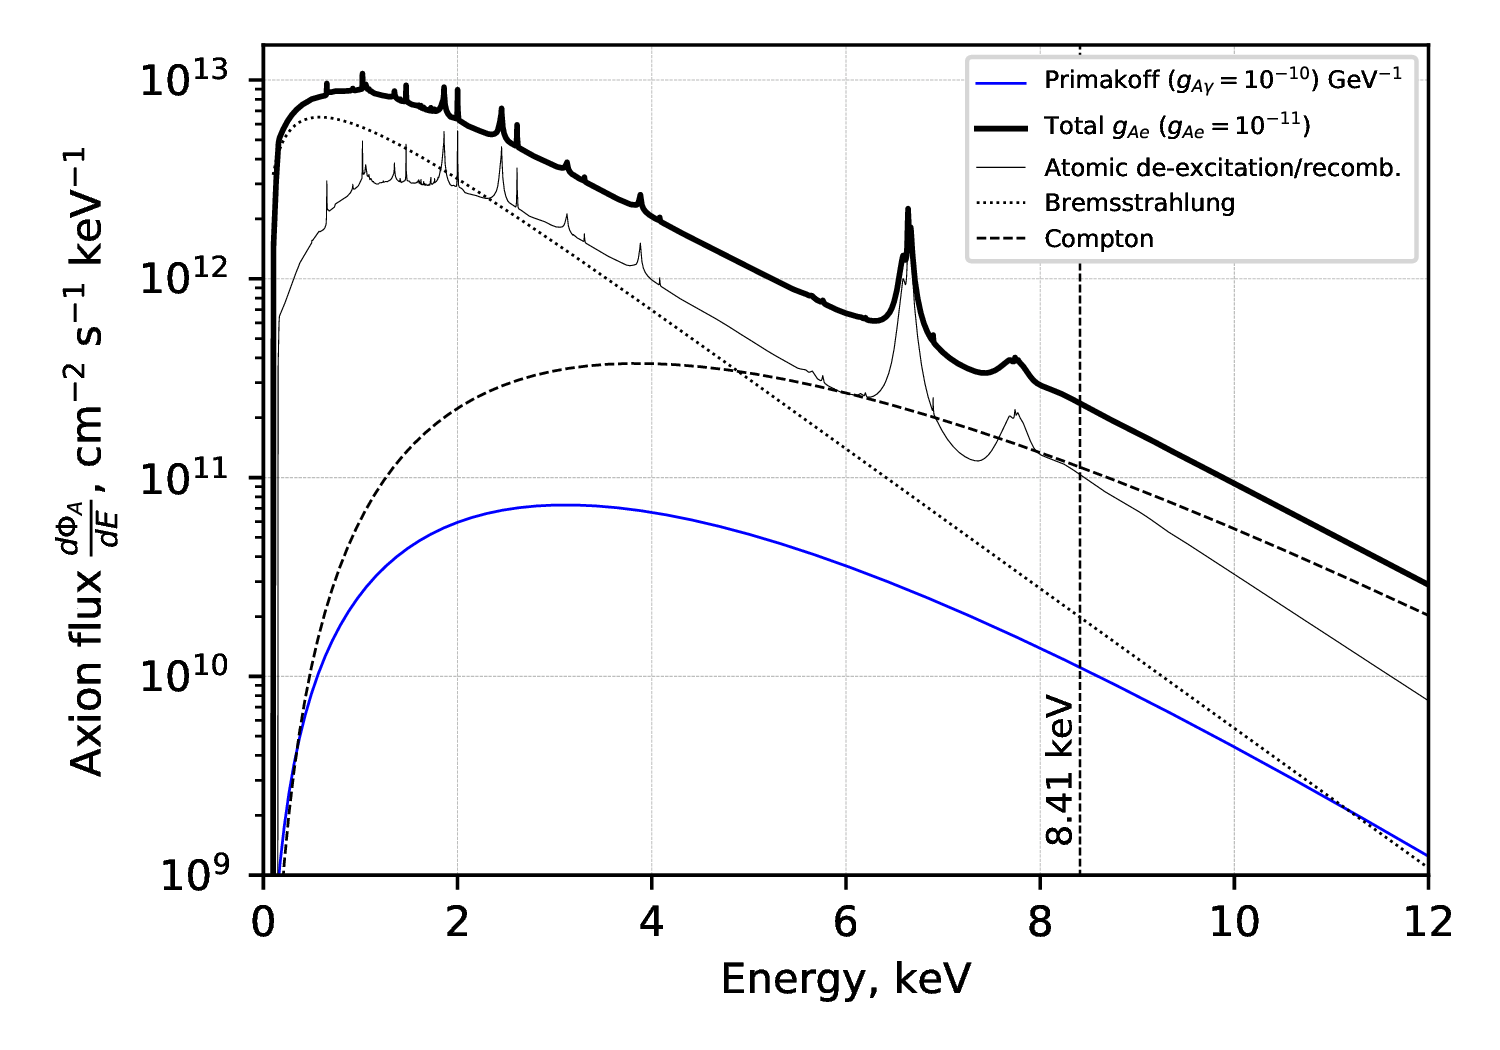
\includegraphics[width = \textwidth]{images/flux_solar.png}
    \caption{Спектр солнечных аксионов}
    \label{flux}
\end{figure}

Воспользовавшись зависимостями \eqref{mA} и \eqref{gAy}, можно получить полный поток аксионов от данного процесса в терминах $m_A$:

\begin{equation}
 {\Phi _A} = \int\limits_0^{ + \infty } {\frac{{d{\Phi _A}}}{{d{E_A}}}d{E_A} } = 7.44 \cdot {10^{11}}\left( {\frac{{{m_A}}}{{1{\text{ эВ}}}}} \right)\left[ {{\text{ \~n }}{{\text{ см}}^{ - 2}}{{\text{ с}}^{ - 1}}} \right]
\end{equation}

Предпринимались попытки обнаружить данные аксионы при конверсии аксиона обратно в фотон в лабораторных магнитных полях (BNL \cite{lazarus1992search}, Tokio axion helioscope \cite{moriyama1998direct,inoue2002search}, CAST - CERN Axion Solar Telescope \cite{beltran2005search}). Кроме того, другой возможный механизм поиска - когерентная конверсия аксиона в фотон в поле кристалла \cite{paschos1994proposal} - лег в основу экспериментов с германиевыми детекторами SOLAX \cite{avignone1998first, avignone1999solar} и COSME \cite{scopel1998theoretical, morales2002particle}, а также DAMA \cite{bernabei2001search} -- с $NaI$ - детектором. Установленные верхние пределы на константу связи варьируются в диапазоне $g_{A \gamma} \leqslant {10^{ - 10}} \div {10^{ - 8}}$.

\subsection{Резонансное поглощение аксиона в ядерных переходах магнитного типа}

Аксион способен испытывать резонансное поглощение атомным ядром в переходах магнитного типа, так как является псевдоскалярной частицей. Релаксация возбужденных ядер приводит к образованию $\gamma$-квантов, а также конверсионых и Оже-электронов, которые детектируются обычными средствами.

Изотопы $^{57}Fe$, $^{83}Kr$, $^{169}Tm$ обладают подходящими низколежащими ядерными переходами для поиска аксиона данным методом. В Петербургском институте ядерной физики активно ведутся эксперименты по поиску резонансного поглощения солнечных аксионов \cite{Derbin2005,Derbin2007,Derbin2009, muratova2015searches, newlimits_tm}

Первые эксперименты были выполнены по схеме «мишень-детектор» c нуклидами $^{57}Fe$ (14.4 кэВ) и $^{169}Tm$ (8.41 кэВ). Расположение мишени -- непосредственно над полупроводниковым Si(Li) детектором. Сама установка находилась на поверхности земли. На сумму изоскалярной $g_{AN}^0$ и изовекторной $g_{AN}^3$ констант связи, а также на произведение данной суммы на $g_{A\gamma}$ были получены следующие ограничения:
\begin{equation}
    Fe:\left| {g_{AN}^3 + g_{AN}^0} \right| \leqslant 3.12 \cdot {10^{ - 6}};\,\,{m_A} \leqslant 151 \text{ эВ}
\end{equation}
\begin{equation}
    Tm:{g_{A\gamma }}\left| {g_{AN}^3 + g_{AN}^0} \right| \leqslant 9.2 \cdot {10^{ - 13}};\,\,{m_A} \leqslant 191 \text{ эВ}
\end{equation}

Следущим шагом было создание низкофоновой установки в сотрудничестве с Баксанской Нейтринной Обсерваторией (БНО) на базе газового пропорционального счётчика \cite{83Kr}. Глубокое расположение (4800 метров водного эквивалента) способствовали чувствительности эксперимента. В установке был использован газообразный криптон, обогащённый изотопом $^{83}Kr$. Предыдущие ограничения были улучшены \cite{Derbin_2017_Kr} и позволили заключить , что:
\begin{equation}
    Kr:\left| {g_{AN}^3 - g_{AN}^0} \right| \leqslant 8.4 \cdot {10^{ - 7}};\,\,{m_A} \leqslant 65 \text{ эВ}
\end{equation}

\subsection{Резонансное поглощение ядрами тулия}

Расмотрим подробнее резонасное поглощение ядром $^{169}Tm$, схема уровней  которого показана на рис. \ref{tmlvls}. Первый ядерный уровень ($3/2^+$) имеет энергию $E = 8.41 \text{ кэВ}$, примесь перехода E2-типа составляет $\delta = 0.033$. Из коэффициента электронной конверсии ($\frac{e}{\gamma} = 285$) \cite{lederer1978table} получается вероятность излучения гамма-кванта $\eta = \frac{1}{1 + \frac{e}{\gamma}} \approx 3.5 \cdot 10^{-3}$

\begin{figure}[h]
    \centering
    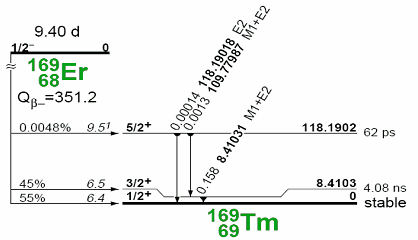
\includegraphics[width = 0.75 \textwidth]{images/Tmlevels.png}
    \caption{Cхема уровней ядра $^{169}Tm$ и вероятнестей преходов на возбуждённые уровни при $\beta$-распаде $^{169}Er$}
    \label{tmlvls}
\end{figure}

Сечение резонансного поглощения аксионов можно получить из выражения для сечения поглощения гамма-квантов, с учётом отношения вероятностей излучения аксиона и фотона $\frac{\omega_A}{\omega _{\gamma}}$ в данном переходе \cite{donnelly1978axions}:

\begin{equation} \label{sech}
    \sigma \left( {{E_A}} \right) =  \pi  {\sigma _{{0_\gamma }}} \Gamma \left( {\frac{{{\omega _A}}}{{{\omega _\gamma }}}} \right)
\end{equation}
\begin{equation} \label{wAwy}
    \frac{{{\omega _A}}}{{{\omega _\gamma }}} = \frac{1}{{2\pi \alpha \left( {1 + {\delta ^2}} \right)}}\frac{{g_{AN}^3 \beta + g_{AN}^0}}{{\left( {\mu_0  - 0.5} \right)\beta  + {\mu_3} - \eta }} \left( {\frac{{{p_A}}}{{{p _\gamma }}}} \right)^3
\end{equation}

где  $\sigma_{0\gamma}$ - максимальное сечение резонансного поглощения гамма-квантов (экспериментально определённое значение для $^{169}Tm$ составляет $\sigma_{0\gamma} = 2.56 \cdot 10^{19} \text{ см}^2$). Из времени жизни первого возбуждённого уровня $\tau = 5.89 \text{ нс}$ можно получить собственную ширину уровня $\Gamma = 1.13 \cdot 10^{-7}$. 

В выражении \eqref{wAwy} $p_A$ и $p_{\gamma}$ - импульсы фотона и аксиона соответственно, $\alpha$ - постоянная тонкой структуры, приблизительно равная $\frac{1}{137}$, $\mu_0 = \mu_p + \mu_n \approx 0.88$ и $\mu_3 = \mu_p - \mu_n \approx 4.71$ - изоскалярный и изовектроный ядерные магнитные моменты. Параметры $\beta$ и $\eta$ задаются ядерными матричными элементами:

\begin{equation}
    \eta  =  - \frac{{\left\langle {{J_f}\left| {\sum\limits_{i = 1}^A {l\left( i \right){\tau _3}\left( i \right)} } \right|{J_i}} \right\rangle }}{{\left\langle {{J_f}\left| {\sum\limits_{i = 1}^A {\sigma \left( i \right){\tau _3}\left( i \right)} } \right|{J_i}} \right\rangle }}
\end{equation}

\begin{equation}
    \beta  =  - \frac{{\left\langle {{J_f}\left| {\sum\limits_{i = 1}^A {\sigma \left( i \right)} } \right|{J_i}} \right\rangle }}{{\left\langle {{J_f}\left| {\sum\limits_{i = 1}^A {\sigma \left( i \right){\tau _3}\left( i \right)} } \right|{J_i}} \right\rangle }}
\end{equation}

и для ядра $^{169}Tm$, имеющего нечётное число нуклонов и неспаренный протон, составляют $\beta \approx 1$ и $\eta \approx 0.5$

Скорость поглощения солнечных аксионов $R_A$ одним ядром $^{169}Tm$ в единицу времени составит:
\begin{enumerate}
    \item[•] в терминах констант связи
    \begin{equation}
    \label{RAg1}
        {R_A} = {C_{Ax}} \cdot g_{Ax}^2{\left( {g_{AN}^0 + g_{AN}^3} \right)^2}{\left( {\frac{{{p_A}}}{{{p_\gamma }}}} \right)^3}
    \end{equation}
    \begin{equation}
        C_{A\gamma } = 104 \qquad C_{Ae} = 2.76 \cdot {10^5}
    \end{equation}
    \item[•] в терминах произведения констант связи и массы
    \begin{equation}
    \label{RAg}
        {R_A} = {C'_{Ax}} \cdot g_{Ax}^2 m_A^2{\left( {\frac{{{p_A}}}{{{p_\gamma }}}} \right)^3}
    \end{equation}
    \begin{equation}
        C_{A\gamma } = 104 \qquad C_{Ae} = 2.76 \cdot {10^5}
    \end{equation}
    \item[•] в терминах массы аксиона
    \begin{equation}
    \label{RAm}
   {R_A} = {C''_{Ax}}m_A^4{\left( {\frac{{{p_A}}}{{{p_\gamma }}}} \right)^3}
\end{equation}
\begin{equation}
        C''_{A\gamma } = 6.64 \cdot 10^{-32} \qquad
        C''_{Ae} = 8.08 \cdot 10^{-31}
    \end{equation}
\end{enumerate}

В приведённых формулах $m_A$ - масса аксиона в эВ. Константы $C_{Ax }$, а также их пересчитанные версии $C'_{Ax }$ и $C''_{Ax }$, зависят от аксионной модели, мишени и др. параметров и были вычислены для ядер $^{169}Tm$ в работах \cite{Derbin2009,redondo2013solar}.



\subsection{Использование тулиевых  болометров}

Работы \cite{Derbin2007,Derbin2009, derbin2011constraints} по поиску аксиона с помощью реакции резонансного поглощения ядром $^{169}Tm$ были выполнены в схеме мишень-детектор. Наилучшие полученные ограничения:

\begin{equation}
    {g_{Ae }}\left| {g_{AN}^3 + g_{AN}^0} \right| \leqslant 2.1 \cdot {10^{ - 14}}
\end{equation}
\begin{equation}
{g_{Ae }} \cdot {m_A} \leqslant 3.1 \cdot {10^{ - 7}} \text{ эВ}
\end{equation}

Внесение вещества мишени в рабочий объём детектора позволяет существенно увеличить чувствительность эксперимента. Нивелируется самопоглощение гамма-квантов веществом мишени. Низколежащие ядерные уровни имеют значительные коэффициенты внутренней конверсии  ($\approx 10^{-2}$), поэтому практически вся энергия рассеивается в детекторе. При этом необходимо достаточно сильное подавление фонов, так как тулий имеет ряд характеристических рентгеновских линий, близких к энергии 8.41 кэВ \cite{Derbin2009}.

Первые попытки задействовать тулийсодержащие кристаллы \\ $NaTm{\left( {W{O_4}} \right)_2}$ и $NaTm{\left( {Mo{O_4}} \right)_2}$ в экспериментах по поиску аксиона были изложены в работе \cite{tm_first}

Использование охлаждённого до 10 мК кристалла тулиевого граната ($Tm_3Al_5O_{12}$) в качестве болометрического криогенного детектора изучено в работе \cite{test_bolometric_tm}. Проведённые измерения подтвердили принципиальную возможность его использования в экспериментах по поиску, тем не менее, указали на ряд сложностей, которые необходимо преодолеть. В частности, радиоактивная чистота сырья должна быть повышена для уменьшения влияния естественной радиоактивности на низкофоновый эксперимент; разрешение детектора также требует оптимизации.

Недавняя работа \cite{newlimits_tm} реализовала описанный эксперимент для тулиевого болометра с датчиком края перехода (Transition Edge Sensor), напыленным непосредственно на поверхность кристалла. Эффективная экспозиция составила 19.2 $\text{г} \cdot \text{день}$. Полученные ограничения:

\begin{equation}
    {g_{A\gamma }}\left| {g_{AN}^3 + g_{AN}^0} \right| \leqslant 1.44 \cdot {10^{ - 14}} \text{ ГэВ}^{-1}
\end{equation}
\begin{equation}
{g_{A\gamma }} \cdot {m_A} \leqslant 2.31 \cdot {10^{ - 7}}
\end{equation}

\begin{equation}
    {g_{Ae }}\left| {g_{AN}^3 + g_{AN}^0} \right| \leqslant 2.81 \cdot {10^{ - 16}}
\end{equation}
\begin{equation}
{g_{Ae }} \cdot {m_A} \leqslant 4.59 \cdot {10^{ - 9}} \text{ эВ}
\end{equation}

Здесь масса аксиона выражена в эВ, $g_{A\gamma }$ в $\text{ ГэВ}^{-1}$, а константы $g_{Ae }$, $g_{AN}^0$ и  $g_{AN}^3$ - безразмерны. Данные ограничения значительно улучшают результаты с тулием в схеме мишень-детектор \cite{Derbin2009}, тем не менее, всё ещё уступая результатам эксперимента с $^{83}Kr$ \cite{Derbin_2017_Kr}.

В настоящее время идёт процесс подготовки к эксперименту в криогенной установке с хорошими низкофоновыми характеристиками. Измерены спектры естественной радиоактивности сырья, выращена новая партия кристаллов тулиевого граната (рис.3). Симуляция данного эксперимента с целью расчёта его чувствительности и является задачей данной работы.


\begin{figure}[h]
    \centering
    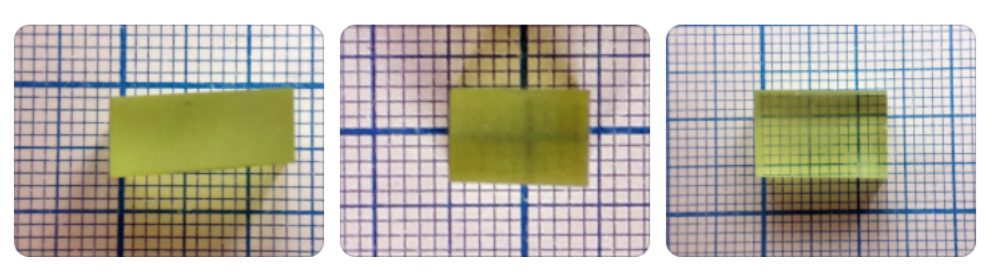
\includegraphics[width = 0.75 \textwidth]{images/Crystals.png}
    \caption{Образцы кристаллов $Tm_3Al_5O_{12}$}
    \label{crystals}
\end{figure}


\newpage 

\section{Оценка параметров симуляции будущего эксперимента по поиску аксионов}
\subsection{Эффективность регистрации HPGe детектора}

Для исследования чистоты сырья, используемого для изготовления тулиевого болометра, были произведены измерения на подземной установке с HPGe-детектором в Баксанской Нейтринной Обсерватории (БНО). Данная установка была промоделирована в Geant4 с целью получения зависимости эффективности регистрации детектора от энергии гамма-частицы, выпускаемой в объёме условного образца.

Схема установки изображена на \ref{geom}:

\begin{figure}[h]
    \centering
    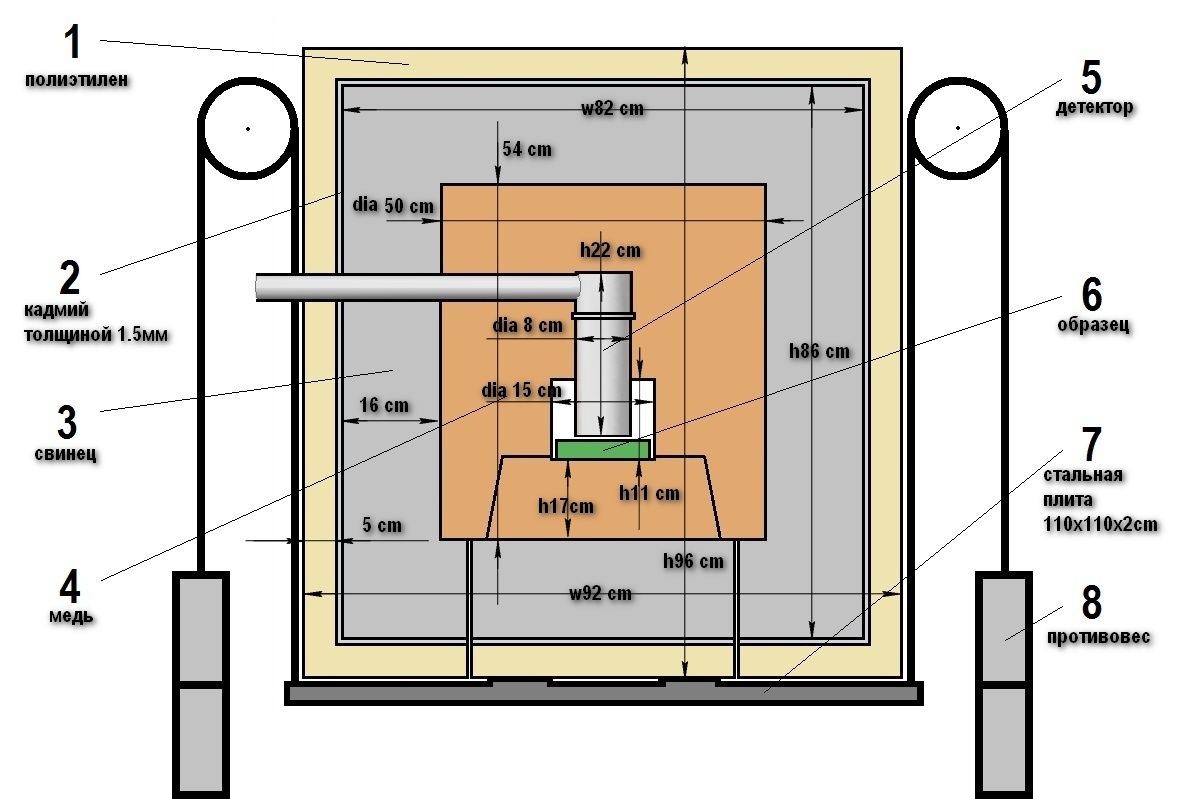
\includegraphics[width = 0.85 \textwidth]{images/farPPD_size.jpg}
    \caption{Геометрические параметры установки farPPD}
    \label{geom}
\end{figure}

Визуализация модели в Geant 4 представлена на \ref{vis}

Вычисленные спектры симуляции:

Чувствительность детектора вычислялась как отношение зарегистрированных событий в пике к полному числу выпущенных частиц:

Исходный код и дополнительная информация доступны \\в репозитории GitHub: \hyperlink{https://github.com/artem-phys/Geant4-farPPD}{https://github.com/artem-phys/Geant4-farPPD}


\subsection{Экспериментальные спектры сырья}
    
    TODO(есть, но их нужно калибровать)
    
\subsection{Экспериментальные спектры фонового излучения}
    Помимо естественного излучения радиоактивных изотопов, содержащихся в сырье для изготовления болометра, учёту также подлежит фоновое излучение внутри будущей установки.
    
    Фоновый спектр (в отсутствие образца) был измерен также на установке farPPD в БНО. Зарегистрированные HPGe-детектором события (рис.1) могут послужить разумной оценкой для моделирования распеределения фонового излучения в симуляции будущего эксперимента по поиску аксиона:
    
    События ниже энергии 50 кэВ не записывались, так как представляют собой шумы регистрации. Ввиду того, что интересующий нас пик 8.41 кэВ находится в указанном диапазоне, возникает необходимость сделать предположения о спектре фонового излучения. К счастью, отсутствие сильных характерных линий в данном диапазоне позволяет ограничится равномерным приближением.
    
\section{Верхний предел на существование аксиона}

\subsection{Моделирование эксперимента}

В качестве базы для конструкции низкофоновой защиты взяты размеры и материалы установки farPPD. Последнее связано исключительно с произвольностью выбора параметров ещё не реализованной установки и не означает, что эксперимент будет реализован на базе farPPD.


Эксперимент моделировался на Geant4 следующим образом:
\begin{enumerate}
    \item Гамма рождаются рандомно
\end{enumerate}
\subsection{Оценка числа возможных аксионных событий}
Slim < чего-то

\subsection{Предел на константы связи}
Найдём число ядер в мишени ${N_{Tm}}$ Для этого вычислим молярную массу вещества детектора:
\begin{equation}
    \mu \left( {T{m_3}A{l_5}{O_{12}}} \right) = 3 \cdot 168.93 + 5 \cdot 26.98 + 12 \cdot 16 = 833.69\frac{\text{г}}{{\text{моль}}}
\end{equation}

Каждая молекула мишени содержит 3 ядра $^{169}Tm$, поэтому

\begin{equation}
    N_{Tm} = 3\nu  \cdot {N_A} = 3\frac{m}{\mu }{N_A} = 3\frac{m}{\mu }{N_A}
\end{equation}

Подставляя $m=
8.18 \text{ г}$, получаем ${N_{Tm}} = 3 \cdot \frac{{8.18}}{{833.69}} \cdot 6.022 \cdot {10^{23}} \approx 1.77 \cdot {10^{22}}$


Полное число зарегистрированных событий в пике, который можно сопоставить с аксионом, пропорционально числу ядер $^{169}Tm$ в мишени, времени измерений и эффективности регистрации детектором. Вероятность зарегистрировать аксионный пик зависит от уровня фона и разрешения детектора. Полагая:
\begin{itemize}
    \item Число ядер в мишени $N_{Tm} = 1.77 \cdot {10^{22}}$
    \item Эффективность регистрации $\varepsilon \sim 1 $, так как в болометрических детекторах ядра мишени находится непосредственно внутри активного объема
    \item Время экспозиции 1 год: $T = 3.15 \cdot {10^7} c$
\end{itemize}

Мы можем записать предел:
\begin{equation}
   \varepsilon  \cdot T \cdot {R_A} \cdot N_{Tm} \leqslant {S_{\lim }}
\end{equation}

Если предположить $\frac{{{p_A}}}{{{p_\gamma}}} \approx 1$, то можно получить ограничение на константы связи, воспользовавшись выражением \eqref{RAg}:

\begin{equation}
     \left| g_{A\gamma}^2{\left( {g_{AN}^0 + g_{AN}^3} \right)^2} \right| \leqslant \frac{{S_{\lim }}}{{C_{Ax}} \cdot \varepsilon  \cdot T \cdot N_{Tm} } 
\end{equation}


\begin{equation}
     \left| g_{Ae}^2{\left( {g_{AN}^0 + g_{AN}^3} \right)^2} \right| \leqslant \frac{{S_{\lim }}}{{C_{Ae}} \cdot \varepsilon  \cdot T \cdot N_{Tm} } 
\end{equation}

\specialsection{Заключение}
Основные результаты, полученные в настоящей работе, заключаются в следующем:

\begin{enumerate}
    \item Разработана модель установки \textit{farPPD} в Geant4
    \item Рассчитана $\varepsilon \left( E_{\gamma} \right)$ -- эффективность регистрации HPGe-детектора, зависящая от энергии гамма-кванта, рождаемого в объёме условного образца
    \item Оценена радиоактивная чистота сырья, используемого для изготовления болометрических кристаллов $Tm_3Al_5O_{12}$
    \item С использованием некоторых деталей конструкции \textit{farPPD} разработана модель будущей низкофоновой установки \textit{TmCryst} в Geant4
    \item Получены экспериментальные спектры симуляции \textit{TmCryst}, с помощью которых рассчитана чувствительность будущего эксперимента по поиску аксиона
    \end{enumerate}

\medskip

\printbibliography[title={Литература}]{}

\end{document}